%
\documentclass{article}
\newcommand{\assgnnum}{5}
\newcommand{\duedate}{February 7}

\usepackage{amsmath}
\usepackage{fullpage}
\usepackage{amssymb}
%\usepackage{bbm}
\usepackage{fancyhdr}
%\usepackage{paralist}
\usepackage{graphicx}
\usepackage{caption}
\usepackage{subcaption}
\usepackage[pdftex,colorlinks=true, urlcolor = blue]{hyperref}
\usepackage{../../arbenson-math}


\oddsidemargin 0in \evensidemargin 0in
\topmargin -0.5in \headheight 0.25in \headsep 0.25in
\textwidth 6.5in \textheight 9in
\parskip 6pt \parindent 0in \footskip 20pt

% set the header up
\fancyhead{}
\fancyhead[L]{CME193: Assignment \assgnnum}
\fancyhead[R]{Due: \duedate}
%%%%%%%%%%%%%%%%%%%%%%%%%%
\renewcommand\headrulewidth{0.4pt}
\setlength\headheight{15pt}

\newcommand{\p}{\ensuremath{\mathbf{P}}}
\renewcommand{\Pr}[1]{\ensuremath{\p \left \{ #1 \right \}}}
\newcommand{\nti}{\ensuremath{n \to \infty}}
\newcommand{\I}{\ensuremath{\operatorname{I}}}
\newcommand{\One}[1]{\ensuremath{\mathbbm{1}_{\left \{ #1 \right \}}}}
\newcommand{\E}{\ensuremath{\mathbf{E}}}
\newcommand{\Ex}[2][]{\ensuremath{\E_{#1} \left[ #2 \right]}}
\newcommand{\var}{\ensuremath{\operatorname{Var}}}
\newcommand{\cov}{\ensuremath{\operatorname{Cov}}}
\newcommand{\F}{\ensuremath{\mathcal{F}}}
\newcommand{\R}{\ensuremath{\mathbb{R}}}
\newcommand{\C}{\ensuremath{\mathbb{C}}}
\newcommand{\NormRV}[2]{\ensuremath{\operatorname{N}\left(#1, #2\right)}}
\newcommand{\BetaRV}[2]{\ensuremath{\operatorname{Beta}\left(#1, #2\right)}}
\newcommand{\argmax}{\operatornamewithlimits{argmax}}
\newcommand{\x}{\mathbf{x}}
\newcommand{\A}{\mathbf{A}}
\newcommand{\bb}{\mathbf{b}}

\newcounter{points}
\setcounter{points}{0}
\newcounter{bonuspoints}
\setcounter{bonuspoints}{0}

\newcommand\setpoints[1]{\addtocounter{points}{#1}(#1 points)}
\newcommand\setpoint{\addtocounter{points}{1}(1 point)}
\newcommand\setbonuspoints[1]{\addtocounter{bonuspoints}{#1}(#1 bonus points)}
\newcommand\setbonuspoint{\addtocounter{bonuspoints}{1}(1 bonus point)}

\newcommand\printpoints{Total number of points: \value{\thepoints}}

\newcommand{\eqD}{\ensuremath{\overset{\mathcal{D}}{=}}}

\setlength{\parindent}{0in}
\usepackage[normalem]{ulem}

\begin{document}

\pagestyle{fancy}
%\vspace*{15pt}

50  points total.  70+\% correctness (35+ points) is needed to pass. Remember: you must pass all assignments to pass the class.   This assignment is due in 2 weeks. Please upload your code and the figure to the course Dropbox.

\begin{enumerate}

\item \textbf{Debugging} \setpoints{10} \\
In this question we are going to use python debugging capabilities to examine the state of a computation 
\vspace{.1in}

To profile each of the statements you will create, use the \texttt{timeit} module. There are many ways to use this module (see
\url{ http://docs.python.org/2.7/library/timeit.html}) but you should only need to use the \texttt{timeit()} function. To time multi-line statements, create the statement using triple quotes. Remember to import the necessary modules and create any necessary objects in the setup phase.

\begin{enumerate}
\item append  to an initially empty list sequentially 
\item create an list of zeros of size 1000 and assign elements sequentially
\item use a list comprehension
\item use the python map function
\item use vectorization (NumPy)
\end{enumerate}


\item \textbf{Data Scraping, NumPy, and SciPy} \setpoints{40}

Recreate the below image of Anscombe's quartet. Scrape the data from
\newline
 \url{http://en.wikipedia.org/wiki/Anscombe%27s_quartet}; do not
 hardcode the values. Turn in both the plot and the code you used to create it (insert your own name, of course). Use less than 100 lines of code.

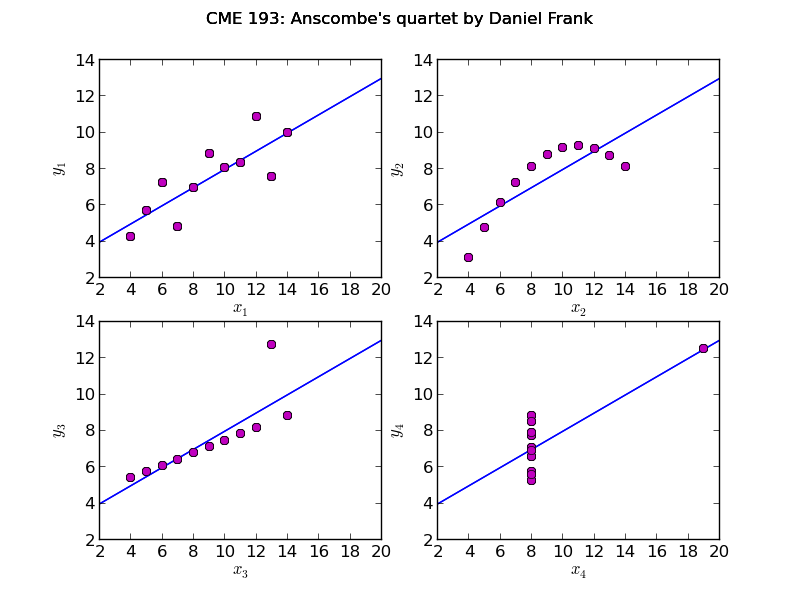
\includegraphics[width=\textwidth]{images/quartet.png}

 

\newpage
\item \textbf{Kernel Density Estimate (KDE)} \setpoints{10}

Given a sample $x_1, x_2, \dots, x_n$ from an unknown distribution $f$ the kernel density estimate of $f$ at point $x$ with kernel $K_b$ is defined as 
$$\hat{f}(x;b) = \frac{1}{n}\sum_{i=1}^{n}K_b(x-x_i)$$
where the kernel must satisfy $\int_{-\infty}^{\infty}K(u)du = 1$ and $K(-u) = K(u).$ The parameter $b$ is known as the bandwidth and controls the width of the kernel used. There are many possible choices for kernels, and we will use the triangular kernel

$$K_{b}(z) = \frac{1}{b}(1 - |\frac{z}{b}|)\mathbb{*I}(|\frac{z}{b} \leq ?1|)$$ 

Write a two line python function \texttt{kde(x, data, bw)} without list comprehension that takes the three parameters below and returns $\hat{f}(x)$, the KDE evaluated at $x$.
\begin{enumerate}
\item \texttt{x} the point to evaluate the KDE
\item \texttt{data}  the sample of points from $f$  ; above denoted $x_1, x_2, \dots, x_n$ 
\item \texttt{bw} the bandwidth of the kernel
\end{enumerate}

\item \textbf{SciPy Optimization} \setpoints{15}

The \texttt{scipy.optimize} module contains functions that perform numerical optimization. Use \newline
\texttt{scipy.optimize.minimize} to minimize the following function. 
$$f(x) = \frac{1}{2}x^TAx - b^Tx$$
When 
A= \begin{pmatrix}
1 & 1\\
1 & 2
\end{pmatrix}
and b = \begin{pmatrix}
1 \\
1 \\
\end{pmatrix}.
Verify that your solution $x^*$ is a solution to the system of linear equations defined by $A$ and $b$. That is, make sure $Ax^*=b$.

\item \textbf{matplotlib} \setpoints{0}

It will be useful to have matplotlib installed for lecture 5. Please install \texttt{matplotlib} on your system and make sure the following lines produce a graph 
\begin{verbatim}
>>> import matplotlib.pyplot as plt
>>> plt.plot(np.arange(10))
>>> plt.show()
\end{verbatim}
\end{enumerate}
%\printpoints.
\end{document} 
